\chapter{Teoretická část}

V teoretické části práce se zaměřím na teoretické principy, na kterých pracují senzory pro monitoring ovzduší. Převážná část z použitých senzorů využívá nepřímý způsob měření námi požadovaných veličin, kde se většinou změna dané veličiny projeví na senzoru změnou odporu a tím i napětí či proudu jím protékajícím.

\section{Měření oxidu uhelnatého}

Oxid uhelnatý je jedovatý plyn bez chuti a zápachu. Vzniká nejčastěji při nedokonalém hoření převážně pevných paliv ale i plynů, proto je třeba jeho hodnotu hlídat. Udává se, že zhruba od 100 ppm je u většiny lidí přítomen nějaký ze symptomů otravy tímto plynem (bolest hlavy, únava, nevolnost).

Oxid uhelnatý lze měřit více způsoby. Nejpřesnější možností je optický senzor využívající infračervené světlo. Tento typ senzoru je založen na základě měření rozdílu intenzity infračerveného záření o dané vlnové délce. Přiváděný plyn je osvětlován infračerveným zářením, které je přítomnými molekulami oxidu pohlcováno a poté je přes reflexní vrstvu odraženo zpět do snímače, kde je umístěn pyrodetektor, který převádí intenzitu tohoto světla na elektrický signál. Se vzrůstající koncentrací klesá intenzita světla dopadajícího na povrch pyrodetektoru. Tento princip měření je nejpřesnější, podává stabilní výsledky a má dlouhou životnost. Bohužel je velice drahý a tak jej není možné použít v domácích zařízeních.

Další z možností měření je elektrochemický senzor. Takovýto senzor pracuje na principu měření proudu vznikajícího reakcí sledovaného plynu s elektrolytem, který je obsažen uvnitř senzoru. Při konstrukci takovéhoto senzoru je třeba zvolit elektrody a elektrolyt tak, aby na jedné z elektrod docházelo k chemické reakci, která vyvolá změnu proudu. Tato změna je poté následně zesílena do měřitelné podoby a odpovídá koncentraci oxidu uhelnatého. Bohužel díky nutnosti chemické reakce několika přítomných látek není tento druh senzoru možné zkonstruovat pro dlouhou životnost. Spolu s tímto neduhem je zde také časová nestálost podávaných výsledků kvůli ubývání elektrolytu a opotřebení měřících elektrod. Životnost takového senzoru je tedy maximálně v řádu několika málo roků. 

Poslední a zároveň nejlevnější možností měření koncentrace oxidu uhelnatého je použití polovodičových senzorů. Polovodičový přechod u těchto senzorů je vyroben tak, aby se při přítomnosti sledovaného plynu změnila jeho vodivost. Na základě této změny jsme poté schopni změřit napětí a proud na přechodu, čímž můžeme určit koncentraci CO. Nevýhodou těchto systémů je ovšem jejich relativní nepřesnost a hlavně nelineární průběh měřeného signálu. Jsou ovšem díky své ceně snadno použitelné a dostupné v komerčně prodávaných detektorech do domácností a pro laická měření. Pro exaktní měření je ovšem nutná jejich častější kalibrace vůči známé koncentraci měřeného plynu.

\section{Měření koncentrace prachových částic}

Prachové částice je možné rozdělit do několika kategorií podle jejich velikosti. Často se lze setkat s pojmem např. PM2.5, což je zkratka z anglického particulate matter (pevné částice) a číslo, které udává maximální velikost těchto částic v \SI{}{\micro\metre}. Nejčastěji se měří částice do velikosti \SI{10}{\micro\metre}, \SI{2,5}{\micro\metre} a \SI{1}{\micro\metre}. Částice o velikosti \SI{10}{\micro\metre} nejsou pro lidský organismus příliš škodlivé, lidské tělo jich většinu dokáže zachytit již při vstupu do dýchacích cest. Problém nastává při vyšší koncentraci částic o velikosti \SI{2,5}{\micro\metre}. Zde již tělo nemá přirozenou obranu a dostávají se tak přímo do plic. Částice menší než \SI{0,5}{\micro\metre} jsou schopny proniknout až do krevního řečiště.

Nejčastěji se v praxi měří koncentrace částic o velikosti \SI{10}{\micro\metre} a \SI{2,5}{\micro\metre}. Všechna zařízení pro měření těchto částic fungují na principu pohlcování či odrážení světelného paprsku. Pro měření je tedy potřeba zdroj světla a detektor světelného paprsku. Jako zdroj se používají LED nebo stále častěji laser. Princip měření tedy spočívá v osvícení vzorku vzduchu daným paprskem světla, který se o prachové částice ve vzorku rozptýlí nebo pohltí. Množství dopadeného světla je tedy nepřímo úměrné koncentraci prachových částic v daném vzorku. V principu jsme schopni měřit tak malé částice, jak přesný zdroj světla (šířka paprsku) jsme schopni vyrobit a také jej potom detekovat.

Dříve používané LED mají nevýhodu v tom, že vyzařují široký paprsek světla, který nejsme schopni jednoduše soustředit do jednoho bodu. Lze využít optickou soustavu pro zaostření takového paprsku světla, ovšem v daném prašném prostředí by docházelo k častému opotřebení a zaprášení čoček, které by poté ztrácely své vlastnosti a měření by bylo nemožné. Z těchto důvodů je v dnešní době více používanější laser, jelikož jsme schopni vytvořit paprsek o dané vlnové délce, výkonové hustotě a velikosti. 

Poslední součástí těchto detektorů je mechanismus, kterým se do senzoru dostává čerstvý vzorek vzduchu. Nejjednodušší je využití malého ventilátoru, který bude do prostoru senzoru vhánět čerstvý vzduch z okolí. Nevýhodou takového řešení je hlučnost senzoru a také možnost zanášení senzoru nečistotami z okolí. Proto se objevují i senzory, které mají tento ventilátor nahrazeny topným elementem (nejčastěji výkonový rezistor), kterým protéká proud a ohřívá vzduch okolo. Ten pak díky rozdílné hustotě teplého a studeného vzduchu začne stoupat vzhůru a unáší s sebou prachové částice do měřeného prostoru. Zde je ovšem třeba dávat pozor na konstrukci takového senzoru a na výrobcem předepsané požadavky na montáž, jelikož jej nelze umístit téměř libovolně v prostoru, jako tomu může být u senzoru s ventilátorem.

\begin{figure}
    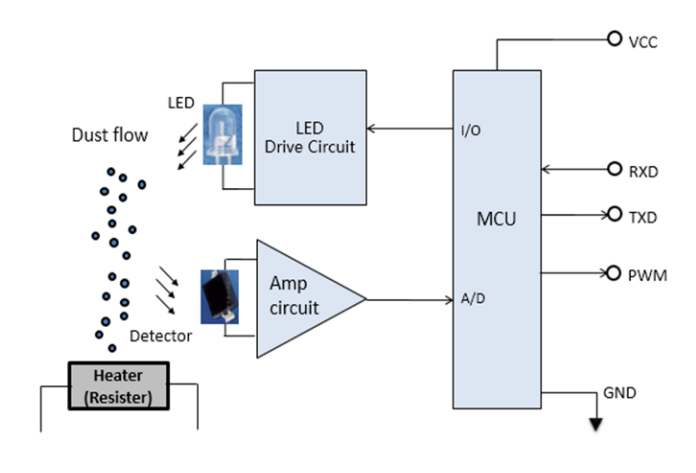
\includegraphics[width=0.70\textwidth]{obrazky/dustSensorPrinciple.png}
    \label{fig_dustSensorPrinciple}
    \caption{Blokové schéma senzoru prachových částic PM1003.}
\end{figure}

\section{Měření intenzity osvětlení}

Intenzita osvětlení se měří na základě fotoefektu. To znamená, že při dopadu elektromagnetického záření na látku dojde k uvolnění elektronů z této látky a naopak k pohlcení fotonů. Nejčastěji se pro tento jev používají polovodiče.

Prvním z používaných typů senzorů jsou fotodiody. U nich se využívá vnitřního fotoelektrického jevu, který je pro polovodiče typický. Dopadem fotonů na PN přechod fotodiody dochází ke zvyšování procházejícího proudu diodou. Tento proud jsme schopni následně měřit a vyhodnocovat. Fotodiody mají výhodu v jejich rychlé odezvě na skokovou změnu a citlivosti.

Dalším často používaným prvkem pro měření intenzity osvětlení jsou fototranzistory. Zde se využívá nejčastěji tranzistor NPN, který má volnou bázi. Při výrobě jsou konstruovány tak, aby dopadající fotony dopadly do oblasti kolektoru a způsobily tak zvýšení protékajícího proudu tranzistorem. Díky tomu, že se díky fotonům řídí proud do báze tranzistoru, tak je tranzistor na světlo více citlivější než fotodioda. Nevýhodou fototranzistoru je shora omezené spektrum detekovaného světla a jeho pomalá reakce.

\section{Měření UV záření}

Měření UV záření probíhá v principu úplně stejně, jako měření intenzity osvětlení. Jediným podstatným rozdílem je vlnová délka záření, na které jsou dané senzitivní součástky nejvíce citlivé. Nejčastěji se vyskytuje UVA záření, které má rozsah vlnových délek mezi \SI{315}{\micro\metre} do \SI{400}{\micro\metre}. Toto záření je zcela běžně přítomné všude kolem nás, jelikož dokáže projít zemskou atmosférou. Při běžném kontaktu s tímto zářením nám nehrozí žádné zdravotní problémy, ale nedoporučuje se trvalejší vystavení tomuto záření. Běžně se také využívá při procesech luminiscence či různých světelných efektech. Lidské oko jako takové jej není schopné vnímat, narozdíl od některých zvířat.

Dalším z UV záření, se kterým se můžeme setkat, je UVB záření s vlnovou délkou od \SI{280}{\micro\metre} do \SI{315}{\micro\metre}. Toto záření je pro živé organismy zhoubné, jelikož dokáže rozkládat bílkoviny. Při dopadu do lidského oka dokáže způsobit oslepnutí, neblahý efekt má též na rostliny, u kterých dokáže ovlivnit fotosyntézu a také způsobit jejich úhyn.

Posledním z těchto záření je UVC záření, které je se svou vlnovou délkou menší než \SI{280}{\micro\metre} nejtvrdším z těchto záření. Při kontaktu s kyslíkem začíná vznikat ozon a je silně karcinogenní pro všechny živé organismy. Díky své krátké vlnové délce dokáže proniknout relativně hluboko do všech organických materiálu a je tak velice nebezpečné.

\section{Měření teploty}

Teplota je základní veličinou, která se dá ve spojitosti s ovzduším měřit. 